
\begin{frame}{Case Studies}
MiniBrass wird für verschiedene Anwendungen eingesetzt:

\vspace*{2ex}

\begin{itemize}
\item \alert<2->{Energiefallstudie}
\item \alert<2->{Studenten-Mentoren-Matching}
\item \alert<2->{Prüfungsterminfindung}
\item \alert<2->{Multi-User-Multi-Display}
\item Rekonfigurierbare Roboterteams
\item Potentiell: Rollenallokation im ODP
\end{itemize}
\end{frame}

\begin{frame}[fragile]{Mentor Matching}

\textbf{Ziel}: Teile Mentees (z.B. Studenten) Mentoren zu (z.B. Firmen), sodass
\begin{itemize}
\item Studenten sind sehr zufrieden mit ihren Mentoren
\item Firmen sind mit ihren Mentees ebenfalls zufrieden
\item Zweiseitige Präferenzen
\end{itemize}

\vspace*{2ex}

Zusätzliche Constraints sind vorhanden:

\begin{itemize}
\item[-] Jede Firme betreut zumindest $l$, höchstens aber $u$ Studenten
\item[-] Die Anzahl betreuter Studenten \emph{sollten} ungefähr gleich sein pro Firma (Fairness)
\item[-] Studenten, die eine Firma ``verachten'', sollen nicht gezwungen werden (\emph{harter Ausschluss} von Lösungen)
\end{itemize}
\end{frame}


\begin{frame}[fragile]{Studenten-Mentoren-Matching: Modell}
\begin{center}

\begin{tikzpicture}[>=stealth',shorten >=1pt,anchor=north west] 

%% FIRST OVERALL LAYER 

\draw[CornflowerBlue,thick,fill=white] (-0.4,0.7) rectangle (9,-6.7);
\node[CornflowerBlue] at (0, 0.6) {$\ltimes \quad \mathtt{lex}$};
\draw[CornflowerBlue,thick] (-0.4,-3.2) -- (9,-3.2);

% the logo

\begin{scope}
\node[pvsNode,minimum width=8.5cm,minimum height=3cm] (outer) at (0,0) {};


\begin{scope}[node distance=.6cm]

\draw [shading=axis,bottom color=black!10,top color=white,rounded corners] (0,0) -- (0,-1) -- (1.3,-1) -- (1.7,0) -- (0,0);
\draw(0,-1) -- ($ (outer.north east) + (0,-1) $);


% constraint relationship logo
\node[cpLogo] (upLogo) at (.55,-.2) {};
\node[cpLogo,below left of=upLogo] (leftLogo) {};
\node[cpLogo,below right of=upLogo] (rightLogo) {};  

\path[->]
  (leftLogo) edge node [right] {} (upLogo)
  (rightLogo) edge node [right] {} (upLogo)
;
\end{scope}

% spd parameter
\begin{scope}[node distance=0.7cm,xshift=3cm,scale=.5,transform shape]

% constraint relationship logo
\node[fill,circle,OliveGreen] (upLogo) at ($ (outer.north east) + (-1.3,-0.2) $) {};
\node[fill,circle,BrickRed,below of=upLogo] (centerLogo) {};
\node[fill,circle,gray,left of=centerLogo] (leftLogo) {};
\node[fill,circle,gray,right of=centerLogo] (rightLogo) {};  
\node[below of=centerLogo,yshift=.4em,font=\Large] {$\mathrm{SPD}$};
\path[->]
  (leftLogo) edge node [right] {} (upLogo)
  (centerLogo) edge node [right] {} (upLogo)
  (rightLogo) edge node [right] {} (upLogo)
;
\end{scope}

% EV
\begin{scope}[node distance=1.2cm]
\node[ anchor=center] at  ($ (outer.center) + (0.2,.9)$) {  $\mathtt{students}$ };


\node[main node, anchor=center,style={font=\sffamily\footnotesize}] (8) at ($ (outer.center) + (0,-0.2)$)   {$\mathtt{raubholzdelphi}$};

\node[main node, style={font=\sffamily\footnotesize},below right of=8,xshift=0.7cm] (4)  {$\mathtt{raubholzyouthlab}$};

\node[main node, style={font=\sffamily\footnotesize},below left of=8] (3) {$\mathtt{raubholzcupg}$};
\end{scope}
%\node[text width=2cm, anchor=west, left] at (4.3, 0.3) { CR };
%\node[text width=1cm, anchor=east, left] at (5.3, -2.3) { \textsc{SPD} };


\path[every node/.style={font=\sffamily\tiny},->]
  (3) edge node [right] {} (8)
  (4) edge node [right] {} (8)
;

\end{scope}


%% SECOND PVS 
%%%%%%%%%%%%%%%%%%%
\begin{scope}[yshift=-3.6cm]
\node[pvsNode,minimum width=8.5cm,minimum height=2.5cm] (outer) at (0,0) {};

% the logo

\begin{scope}[node distance=.6cm]

\draw [shading=axis,bottom color=black!10,top color=white,rounded corners] (0,0) -- (0,-1) -- (1.3,-1) -- (1.7,0) -- (0,0);
\draw(0,-1) -- ($ (outer.north east) + (0,-1) $);


% constraint relationship logo
\node[cpLogo] (upLogo) at (.55,-.2) {};
\node[cpLogo,below left of=upLogo] (leftLogo) {};
\node[cpLogo,below right of=upLogo] (rightLogo) {};  

\path[->]
  (leftLogo) edge node [right] {} (upLogo)
  (rightLogo) edge node [right] {} (upLogo)
;
\end{scope}

% spd parameter
\begin{scope}[node distance=.7cm,xshift=3cm,scale=.5,transform shape]

% constraint relationship logo
\node[fill,circle,OliveGreen] (upLogo) at ($ (outer.north east) + (-1.3,-0.2) $) {};
\node[fill,circle,BrickRed,below of=upLogo] (centerLogo) {};
\node[fill,circle,gray,left of=centerLogo] (leftLogo) {};
\node[fill,circle,gray,right of=centerLogo] (rightLogo) {};  
\node[below of=centerLogo,yshift=.4em,font=\Large] {$\mathrm{SPD}$};
\path[->]
  (leftLogo) edge node [right] {} (upLogo)
  (centerLogo) edge node [right] {} (upLogo)
  (rightLogo) edge node [right] {} (upLogo)
;

\end{scope}

% BIOGAS Plant 
\begin{scope}[node distance =0.8cm]
\node[main node, anchor=center, style={font=\sffamily\footnotesize}] (gf) at ($ (outer.center) + (0,0)$) {$\mathtt{delphirich}$};
\node[main node, style={font=\sffamily\footnotesize}] (ecs) [below  of=gf] {$\mathtt{delphikill}$};
\node[main node, style={font=\sffamily\footnotesize}] (ono) [right of=ecs,xshift=1.4cm] {$\mathtt{kasokyouth}$};
\end{scope}
%\node[main node, style={font=\sffamily\footnotesize},double] (hardConstraint) [below left of=7,xshift=-3.1,yshift=7] {$\mathsf{maxProd}$};
\node[ anchor=center] at  ($ (outer.center) + (0.2,.7)$) {  $\mathtt{companies}$ };


%\node[text width=2cm, anchor=west, left] at (4.3, 0.3) { CR };
%\node[text width=1cm, anchor=east, left] at (5.3, -2.3) { \textsc{SPD} };


\path[every node/.style={font=\sffamily\tiny},->]
  (ecs) edge node [right] {} (gf)
;

\end{scope}
\end{tikzpicture}
\end{center}
\end{frame}

\begin{frame}[fragile]{Studenten-Mentoren-Matching: Code}
\begin{lstlisting}
PVS: students = new ConstraintPreferences("students") {
   soft-constraint raubholzdelphi: 'worksAt[raubholz] = delphi';
   soft-constraint raubholzyouthlab: 'worksAt[raubholz] = youthlab';
   soft-constraint raubholzcupg: 'worksAt[raubholz] = cupgainini';
   
   crEdges : '[| mbr.raubholzyouthlab, mbr.raubholzdelphi | 
                 mbr.raubholzcupg, mbr.raubholzdelphi |]';
   useSPD: 'true' ;
}; 

PVS: companies = new ConstraintPreferences("companies") {
   soft-constraint delphi_kill: 'worksAt[kill] = delphi';
   soft-constraint delphi_rich: 'worksAt[rich] = delphi';
   soft-constraint kasokyouth: 'worksAt[kasok] = airtrain';
   
   crEdges : '[| mbr.delphi_kill, mbr.delphi_rich |]';
   useSPD: 'true' ;
}; 

solve students lex companies;
% solve companies lex students;
\end{lstlisting}
\end{frame}

\begin{frame}{Wann Constraint Preferences?}
\alert{Pro}:

\begin{itemize}
\item Wünschenswerte Bedingungen als boolesche Eigenschaften (``Constraints'')
\item Nicht alle erfüllbar
\item Nicht alle \textbf{vergleichbar}
\item \alert{Komparative} Bewertung möglich (``A ist mir wichtiger als B'')
\end{itemize}

\vspace*{2ex}
\hSecond{Contra}:

\begin{itemize}
\item Problem hat numerisches Ziel (Kosten, Verletzungen als Metrik)
\item Feingranulares Tuning für Gewichte von Constraints nötig
\item Ich will nur \emph{eine} Lösung am Ende.
\end{itemize}
\end{frame}

%% Weighted CSP and CFN 
\begin{frame}[fragile]{Prüfungstermine}

\textbf{Ziel}: Weise Prüfungstermine an Studenten zu, sodass
\begin{itemize}
\item Jeder Student stimmt seinem Termin zu 
\item Die Anzahl verschiedener Termine wird minimiert (um das Zeitinvestment der Dozenten zu schonen)
\end{itemize}

%\vspace*{2ex}
%\begin{parchment}
\begin{center}

\includegraphics[width=.15\textwidth]{img/voting.png}
\hspace*{4ex}
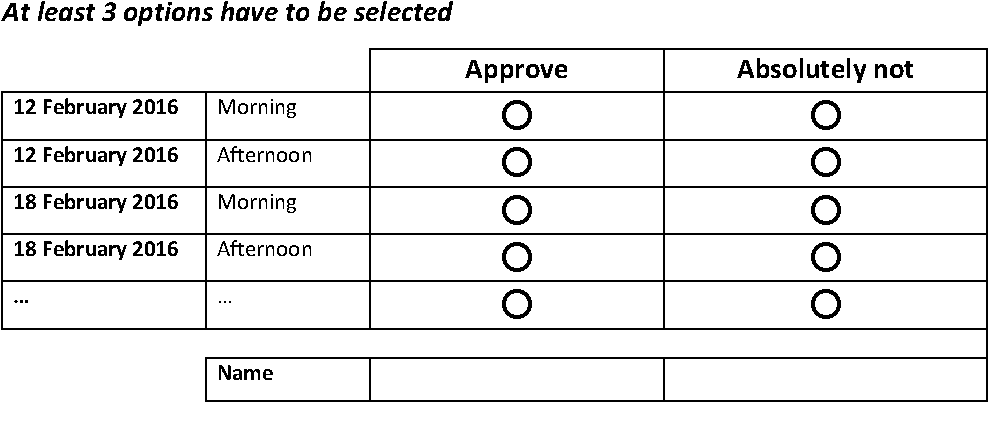
\includegraphics[width=.5\textwidth]{img/Voting.pdf}
\end{center}
%\end{parchment}

\begin{itemize}
\item Kein studentischer Wunsch sollte höher gewichtet werden
\item Prüfungsplan ist eine gemeinsame Entscheidung

\end{itemize}
\end{frame}

\begin{frame}[fragile]{Prüfungstermine: Modell}
\begin{center}
\begin{tikzpicture}[>=stealth',shorten >=1pt,anchor=north west] 

\draw[CornflowerBlue,thick,fill=white] (-0.4,0.7) rectangle (8,-6.7);
\node[CornflowerBlue] at (0, 0.6) {$\ltimes \quad \mathtt{lex}$};
\draw[CornflowerBlue,thick] (-0.4,-3.2) -- (8,-3.2);

\begin{scope}
\node[pvsNode,minimum width=7.5cm,minimum height=3cm] (outer) at (0,0) {};

% the logo

\begin{scope}[node distance=.6cm]

\draw [shading=axis,bottom color=black!10,top color=white,rounded corners] (0,0) -- (0,-1) -- (1.3,-1) -- (1.7,0) -- (0,0);
\draw(0,-1) -- ($ (outer.north east) + (0,-1) $);


% weighted constraints%s logo
\coordinate (beginLogo) at (0.4,0.0);
\node[cpLogo,anchor=south,scale=.8] (upLogo) at ($(beginLogo)+(0.3,-.45)$) {};

\draw [fill=black] ($(beginLogo)+(0,-.7)$) -- ($(beginLogo)+(0.1,-.4)$) -- ($(beginLogo)+(0.5,-.4)$) -- ($(beginLogo)+(0.6,-.7)$) -- ($(beginLogo)+(0,-.7)$);

\begin{scope}[scale=.6, transform shape]
\node[font=\Huge,anchor=east] at ($(outer.east) + (-1.1,1.8)$) {$100$};
\node[font=\Large,anchor=east] at ($(outer.east) + (-1.1,1.2)$) {$\mathrm{maxWeight}$};
\end{scope}
\end{scope}

\node[ anchor=center] at  ($ (outer.center) + (0.2,.7)$) {  $\mathtt{students}$ };

\node[weightNode,text=white,anchor=west,text width=1.5cm,text height=.17cm,align=right] (bg) at ($ (outer.center) + (-2,0.1)$)   {\hfill 1};
\node[main node,draw,anchor=west] (limitBu) at ($ (outer.center) + (-2,0.1)$)   {$\mathtt{meerfluss}$};

\node[weightNode,text=white,anchor=west,text width=1.3cm,text height=.17cm,align=right] (bg2) at ($(limitBu.west)+(0,-.5)$)   {\hfill 1};
\node[main node, anchor=west, style={font=\sffamily\footnotesize}] (earlyBird) at ($(limitBu.west)+(0,-.5)$)  {$\mathtt{ayman}$};

\node[weightNode,text=white,anchor=west,text width=1.3cm,text height=.19cm,align=right] (bg3) at ($(earlyBird.west)+(0,-.5)$)   {\hfill 1};
\node[main node, anchor=west, style={font=\sffamily\footnotesize}] (prefBatteryLevel) at ($(earlyBird.west)+(0,-.5)$)  {$\mathtt{kanye}$};

\node[weightNode,text=white,anchor=west,text width=1.4cm,text height=.17cm,align=right] (bg) at ($ (outer.center) + (1,0.1)$)   {\hfill 1};
\node[main node,draw,anchor=west] (limitBu) at ($ (outer.center) + (1,0.1)$)   {$\mathtt{raubholz}$};

\node[weightNode,text=white,anchor=west,text width=1.7cm,text height=.17cm,align=right] (bg2) at ($(limitBu.west)+(0,-.5)$)   {\hfill 1};
\node[main node, anchor=west, style={font=\sffamily\footnotesize}] (earlyBird) at ($(limitBu.west)+(0,-.5)$)  {$\mathtt{schraubale}$};

\node[weightNode,text=white,anchor=west,text width=2.3cm,text height=.19cm,align=right] (bg3) at ($(earlyBird.west)+(0,-.5)$)   {\hfill 101};
\node[main node, anchor=west, style={font=\sffamily\footnotesize}] (prefBatteryLevel) at ($(earlyBird.west)+(0,-.5)$)  {$\mathtt{kanye-urlaub}$};


\end{scope}

%% SECOND PVS 
%%%%%%%%%%%%%%%%%%%
\begin{scope}[yshift=-3.6cm]
\node[pvsNode,minimum width=7.5cm,minimum height=2.5cm] (outer) at (0,0) {};

% the logo

\begin{scope}[node distance=.6cm]

\draw [shading=axis,bottom color=black!10,top color=white,rounded corners] (0,0) -- (0,-1) -- (1.3,-1) -- (1.7,0) -- (0,0);
\draw(0,-1) -- ($ (outer.north east) + (0,-1) $);


\node at (.1,-.3) {\Huge \EUR};
\node at (.6,-0.1) {\Large $\mathbb{Z}$};


\end{scope}

% spd parameter
\begin{scope}[node distance=.7cm,xshift=3cm,scale=.5,transform shape]

% cfn logos
\draw[thick,->] ($(outer.east) + (-1.3,2)$) -- ($(outer.east) + (-1.3,1)$);
\node[font=\Large,anchor=east] at ($(outer.east) + (-0.5,0.9)$) {$\mathrm{Minimize}$};


\node[font=\Huge,anchor=east] at ($(outer.east) + (-2.7,1.5)$) {$\mathrm{\sum}$};
\node[font=\Large,anchor=east] at ($(outer.east) + (-2.7,0.9)$) {$\mathrm{Sum}$};

\end{scope}

% BIOGAS Plant 
\begin{scope}[node distance =0.8cm]
\node[main node, anchor=center, style={font=\sffamily\footnotesize}] (gf) at ($ (outer.center) + (0,-.5)$) {$\mathtt{scheduledDates}$};
\end{scope}
%\node[main node, style={font=\sffamily\footnotesize},double] (hardConstraint) [below left of=7,xshift=-3.1,yshift=7] {$\mathsf{maxProd}$};
\node[ anchor=center] at  ($ (outer.center) + (0.2,.7)$) {  $\mathtt{teachers}$ };
\end{scope}
\end{tikzpicture}
\end{center}

\end{frame}

\begin{frame}[fragile]{Prüfungstermine: Code}

\begin{lstlisting}
PVS: students = new WeightedCsp("students") {
   maxWeight: '100';
   soft-constraint raubholz:   'sd[raubholz] in {monday, tuesday}';   
   soft-constraint schraubale: 'sd[schraubale] in {tuesday, wednesday}';
   soft-constraint meerfluss:  'sd[meerfluss] in {tuesday}';
   soft-constraint ayman:   'sd[ayman] in {monday, tuesday}';
   soft-constraint kanye:     'sd[kanye] in {monday, wednesday}';
   % hard by weight (less than bottom)
   soft-constraint kanye-urlaub: 'sd[kanye] != tuesday'
                                :: weights('101'); 
}; 
PVS: teachers = new CostFunctionNetwork("teachers") {
   soft-constraint scheduledDates: 'scheduledDates';
}; 
solve students lex teachers;
\end{lstlisting}

\begin{Verbatim}[fontsize=\small]
Scheduled: [1, 2, 2, 1, 1], Distinct dates: 2
Valuations: mbr_overall_students = 0; mbr_overall_teachers = 2
\end{Verbatim}
\end{frame}

\begin{frame}{Wann Weighted CSP / Cost Function Networks?}
\alert{Pro}:

\begin{itemize}
\item Feintuning von Gewichten für Soft Constraints (evt. erlernt vom Benutzer)
\item Skalare Kostenfunktion ist offensichtlich (Produktionskosten, Spanne der Task-Zuweisung) 
\item Fehler können per Distanz angegeben und minimiert werden (50 KW Abweichung ist schlimmer als 10 KW Abweichung)
\item Lösungszeit ist kritisch -- keine Auswahlmöglichkeiten nötig
\end{itemize}

\vspace*{2ex}
\hSecond{Contra}:

\begin{itemize}
\item Es gibt tatsächlich unvergleichbare Kriterien.
\item Ich will mir für eine Ordnung keine Gewichtung ``ausdenken'' müssen -- besonders wenn sich Soft Constraints häufig ändern.
\item Viele Entscheidungsvarianten gewünscht (nicht nur ``skalares Optimum'') -- z.B. in Offline-Entscheidungssituationen
\end{itemize}
\end{frame}

\begin{frame}[fragile]{Probabilistic Constraints \cite{fargier1993uncertainty}}
\begin{figure}[t]
\centering
\begin{tikzpicture}[>=stealth',shorten >=1pt,anchor=north west] 


\begin{scope}
\node[pvsNode,minimum width=4cm,minimum height=3cm] (outer) at (0,0) {};

% the logo

\begin{scope}[node distance=.6cm]

\draw [shading=axis,bottom color=black!10,top color=white,rounded corners] (0,0) -- (0,-1) -- (1.3,-1) -- (1.7,0) -- (0,0);
\draw(0,-1) -- ($ (outer.north east) + (0,-1) $);

% probabilistic constraints%s logo

\node at (1,-0.1) {\Large $\mathbb{P}$};
\draw(0.7,-0.3) -- (0.7,-.9);
\draw(0.3,-0.7) -- (1.1,-.7);

\draw [thick] plot [smooth, tension=.6] coordinates {(0.3,-0.59) (0.55,-0.59) (0.7,-0.39)  (0.85,-0.59) (1.1,-0.59) };

\end{scope}

\node[main node,draw,anchor=west] (limitBu) at ($ (outer.center) + (-1,0.1)$)   {\texttt{beerSupp}};

\node[main node, anchor=west, style={font=\sffamily\footnotesize}] (prefBatteryLevel) at ($(limitBu.west)+(1.2,-.6)$)  {\texttt{beerDem}};


\end{scope}

\end{tikzpicture}
\end{figure}
\begin{lstlisting}
type ProbabilisticConstraints = PVSType<bool, 0.0 .. 1.0> = 
  params {
    array[1..nScs] of float: probs :: default('1.0');
  } in  
  instantiates with "soft_constraints/mbr_types/probabilistic_type.mzn" {
    times -> prod;
    is_worse -> is_worse_prob;
    top -> 1.0;
};   
[...]
soft-constraint beerDem: 'dem1 + dem2 >= 10' :: probs('0.7');
soft-constraint beerSupp: 'sup1 + sup2 <= 10' :: probs('0.2');
\end{lstlisting}
\end{frame}

\begin{frame}{Wann Probabilistic Constraints?}
\alert{Pro}:

\begin{itemize}
\item Wenn ich unsicher bin, ob ein Constraint wirklich vorhanden sein wird.
\item Wenn ich die Wahrscheinlichkeit wissen will, dass \emph{alle} (vl. noch nicht sicheren) Constraints erfüllt sind
\item Weighted Variante straightforward
\end{itemize}

\vspace*{2ex}
\hSecond{Contra}:

\begin{itemize}
\item Andere Verteilungen außer ``Münzwurf'' nicht behandelt (Constraint gilt oder nicht)
\item Bildet keine Szenarien ab
\item Eignet sich nicht für einen erwarteten Kostenwert
\end{itemize}
\end{frame}

\begin{frame}[fragile]{Fuzzy Constraints \cite{ruttkay1994fuzzy}}
\begin{figure}[t]
\centering
\begin{tikzpicture}[>=stealth',shorten >=1pt,anchor=north west] 


\begin{scope}
\node[pvsNode,minimum width=4cm,minimum height=3cm] (outer) at (0,0) {};

% the logo

\begin{scope}[node distance=.6cm]

\draw [shading=axis,bottom color=black!10,top color=white,rounded corners] (0,0) -- (0,-1) -- (1.3,-1) -- (1.7,0) -- (0,0);
\draw(0,-1) -- ($ (outer.north east) + (0,-1) $);

\node at (1,-0.1) {\Large $\mathrm{\mu}$};


\draw(0.4,-0.1) -- (0.4,-.8);
\draw(0.3,-0.7) -- (1.2,-.7);
\node[scale=0.5,transform shape,anchor=east] at (0.35,-0.6) {0};
\node[scale=0.5,transform shape,anchor=east] at (0.35,-0.25) {1};

\draw [thick] plot [smooth, tension=.2] coordinates { (0.4,-0.59) (0.6,-0.59) (0.85,-0.25)(1.05,-0.25)};

\end{scope}

\begin{scope}[node distance=.7cm,xshift=1.7cm,scale=.5,transform shape]

%\node[font=\Huge] at (2.7,-0.3) {$\mathrm{\Min}$};
%\node[font=\Large] at (2.6,-1.3) {$\mathrm{Minimum}$};

\end{scope}
\node[main node,draw,anchor=west] (limitBu) at ($ (outer.center) + (-1,0.1)$)   {\texttt{taste1}};

\node[main node, anchor=west, style={font=\sffamily\footnotesize}] (earlyBird) at ($(limitBu.west)+(1,-.8)$)  {\texttt{taste2}};



\end{scope}

\end{tikzpicture}
\end{figure}

\begin{lstlisting}
type FuzzyConstraints = PVSType<0.0 .. 1.0> = 
  instantiates with "soft_constraints/mbr_types/fuzzy_type.mzn" {
    times -> min;
    is_worse -> is_worse_fuzzy;
    top -> 1.0;
};
PVS: fz1 = new FuzzyConstraints("fz1") {
   soft-constraint taste1: 'fbinary_fuzzy([1.0, 0.8, 0.3, 0.7], main, wine)';
   soft-constraint taste2: 'fbinary_fuzzy([1.0, 0.8, 0.8, 1.0], main, dessert)';
}; 
solve fz1;
\end{lstlisting}
\end{frame}

\begin{frame}{Wann Fuzzy Constraints?}
\alert{Pro}:

\begin{itemize}
\item Wenn ich Kombinationen (z.B. Essen+Wein) als Zufriedenheitsprozentsatz ausdrücken will.
\item Wenn Soft Constraints relativ formuliert werden kann (als Verhältnis), z.B. \texttt{supply / Demand}  
\item Einfach zu interpretierender, einzelner Erfüllungsgradwert (0.7 bedeutet, der \emph{schlechteste} Soft Constraint bildet  auf 0.7 ab)
\end{itemize}

\vspace*{2ex}
\hSecond{Contra}:

\begin{itemize}
\item Sehr strenge Semantik bei Abbildung auf geringsten Wert 
\item Floating Point Unterstützung in Constraint Solvern dürftig (daher besser nach Weighted CSP mit Morphismus abbilden)
\end{itemize}
\end{frame}